\subsection{Glyph: \glyph{Necessary stimulation}}
\label{sec:af:trigger}
A \glyph{necessary stimulation} is an influence that has to be present for the target activity to take place (to become true).  An activity modulated by a necessary stimulation can only exist when this stimulation is true, whatever are the other influences this activity is subjected to.

\begin{glyphDescription}

\glyphSboTerm SBO:0000171 ! necessary stimulation

 \glyphOrigin Any \glyph{Activity node} (\sect{af:ANs}) or any \glyph{logical operator} (\sect{af:logic}).
 \glyphTarget Any \glyph{biological activity} or \glyph{phenotype} (\sect{af:ANs}).
 \glyphEndPoint The target extremity of a \glyph{necessary stimulation} carries a perpendicular bar followed by an open arrow pointing to the target activity node (\fig{af:trigger}).

\end{glyphDescription}

\begin{figure}[H]
  \centering
  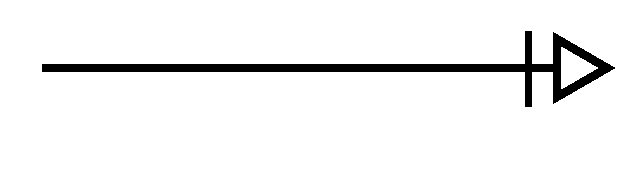
\includegraphics[width = 2in]{images/necessaryStimulation}
  \caption{The \AF glyph for \glyph{necessary stimulation}.}
  \label{fig:af:trigger}
\end{figure}

\begin{figure}[H]
  \centering
  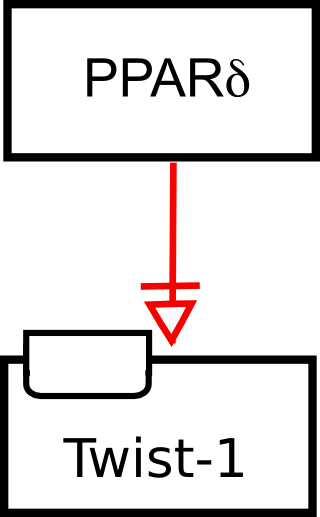
\includegraphics[width = 1.5in]{examples/ex-necessaryStimulation}
  \caption{An example of \glyph{necessary stimulation} where nuclear hormone receptor \glyph{PPAR $\delta$} transcription factor activity stimulates the gene expression of \glyph{Twist-1}. }
  \label{fig:af:ex-NS}
\end{figure}
